\section{Begriffserläuterung}
Ein Einstieg in das Thema lässt sich durch die Definition der beiden Begriffe ,,Business Intelligence`` und ,,Data Warehouse`` finden. 

\begin{description}
	\item[Business Intelligence] ist ein ,,Sammelbegriff für den IT-gestützten Zugriff auf Informationen, sowie die IT-gestützte Analyse und Aufbereitung dieser Informationen. Ziel dieses Prozesses ist es, aus dem im Unternehmen vorhandenen Wissen, neues Wissen zu generieren. Bei diesem neu gewonnenen Wissen soll es sich um relevantes, handlungsorientiertes Wissen handeln, welches Managemententscheidungen zur Steuerung des Unternehmens unterstützt.`` \\ \href{http://wirtschaftslexikon.gabler.de/Definition/business-intelligence.html}{[http://wirtschaftslexikon.gabler.de]}
	\item [Data Warehouse bzw. Business Warehouse] ist eine ,,von den operativen Datenverarbeitungssystemen separierte Datenbank, auf die nur Lesezugriff besteht. In regelmäßigen Abständen werden aus den operativen DV-Systemen unternehmensspezifische, historische und daher unveränderliche Daten zusammengetragen, vereinheitlicht, nach Nutzungszusammenhängen geordnet, verdichtet und dauerhaft in der Datenbasis des Data Warehouses archiviert. Ziel ist die Verbesserung der unternehmensinternen Informationsversorgung (Wissensmanagement) und damit der Unterstützung strategischer Entscheidungen. Als analytisches System liefert es Informationen zur Problemanalyse - Online Analytical Processing (OLAP) -, die durch die Anwendung von Methoden (z.B. des Data Mining) generiert werden.`` \\ 
	 		\href{http://wirtschaftslexikon.gabler.de/Definition/data-warehouse.html?referenceKeywordName=Business+Warehouse}{[http://wirtschaftslexikon.gabler.de]}
\end{description}

Nach dieser Definition ist Data Warehouse kein allein stehendes Produkt, sondern ein Konzept, durch das die Datenproblematik im Bereich Business Intelligence  angegangen bzw. gelöst werden soll. Die Firma SAP hat sich diesem Problem angenommen und stellt mit der Data Warehousing Workbench ein kostenpflichtiges Tool bereit mit dem sich Aufgaben im Data Warehouse Bereichen lösen lassen können.  \\
Diese eine Definition alleine ist aber nicht ausreichend. Einen genaueren bzw. verständlicheren Einblick gibt W.H. Inmon. ,,A data warehouse is a subject oriented, integrated, non-volatile, and time variant collection of data in support of management\'s decisions`` \cite[S. 33]{Inmon:2005vg}. Seiner Meinung nach muss ein Data Warehouse themenorientiert, integriert, nicht flüchtig und zeitbezogen sein. Dies bedeutet im Zusammenhang: \\
\begin{description}
	\item [1. Themenorientiert (engl. subject oriented)] bedeutet, dass Prozesse im Unternehmen durch Kennzahlen wie Kosten und Umsätze abgebildet werden sollen. Es reicht dabei nicht aus, dass das System nur die Berechnungen durchführt. Die Ergebnisse müssen zusätzlich ihrem spezifischen Themenbereich zugeordnet werden. 
	\item [2. Itegriert (engl. integrated)] bedeutet, dass Daten aus den verschiedensten Quellen und Fremdsystemen verwendet werden können. So können die unterschiedlichsten Daten in Verbindung miteinander gebracht werden und neue Ergebnisse liefern.
	\item [3. Nicht flüchtig (engl. non-volatile)]bedeutet, dass Daten, sofern sie einmal im Data Warehouse abgelegt worden sind nicht gelöscht oder modifiziert werden dürfen. Korrekturen sind die Ausnahmeregelung. Denn so ist es möglich Auswertungen über längere Zeiträume durchzuführen.
	\item [4. Zeitbezogen (engl. time variant)] bedeutet, dass Daten in der Regel Zeitpunkte zugeteilt sind, da alle Daten sozusagen immer nur ein Schnappschuss einer Situation im Unternehmen sind und daher eindeutig zugeordnet werden können.
\end{description}


%1. Die Themenausrichtung an Sachverhalten des Unternehmens, z.B. Kunden- oder Produktkriterien, wird im BW durch das konsequente Einordnen aller Daten in Fachbereiche und durch die Bezugnahme auf Geschäftsprozesse realisiert (Seemann/Schmalzridt/Lehmann 2001, 18). Im Gegensatz dazu sind operative Daten immer auf einzelne betriebliche Funktionen bezogen (Schinzer/Bange/Mertens 1999, 14 - Bange/ Schinzer o.J., 1). \\


%2. integrated: Mit dem DW-Konzept wird eine unternehmensweite Integration von Daten in einem einheitlich gestalteten System angestrebt (Mucksch/Behme 2000, 11). Verein- heitlichung und Integration externer und interner Daten bedeutet weniger die physische Zentralisierung der Daten in einem einzigen Datenpool, sondern deren logische Ver- bindung. Integration bedeutet konsistente Datenhaltung im Sinne einer Struktur- und Formatvereinheitlichung durch Maßnahmen wie Vergabe eindeutiger Bezeichnungen, Anpassung der Datenformate und Herstellung einer semantischen Integrität (Mucksch/ Behme 2000, 11ff.). Ebenso tragen Elemente wie einheitliche Merkmale und standardi- sierte Kennzahlen zu einer Datenintegration bei.\\
%3. nonvolatile: Bei einem DW handelt es sich um eine dauerhafte Sammlung von Informationen, auf die im Gegensatz zu OLTP-Systemen (online transaction processing3) nur in Form von Lese- und Einfügeoperationen zugegriffen werden darf, um die Nicht- Volatilität der Daten sicherzustellen.4 Dieser Forderung kann jedoch nur bedingt zuge- stimmt werden, da Korrekturen von aus Quellsystemen geladenen Daten auf jeden Fall möglich sein müssen (Behme 1996, 31). Das BW bietet hierfür eine Eingangsablage in Form der Persistent Staging Area (PSA)5, in der manuelle Korrekturen zur Validierung und Fehlerbehebung nach dem Extraktionsvorgang durchgeführt werden können (SAP 2000a, 1; SAP 2000b).\\
%4. time-variant: Während bei operativen Systemen eine zeitpunktgenaue Betrachtung der Daten im Mittelpunkt steht, liegt das Interesse bei Auswertungen im DW eher in einer Zeitraumbetrachtung, z.B. einer Trendanalyse (Behme 1996, 31). Der Zeitraumbezug ist daher impliziter oder expliziter Bestandteil der Daten in einem DW. Ein Ansatz zur Herstellung dieses Zeitraumbezugs im BW ist die obligatorische Verwendung einer Zeitdimension in jedem Informationsspeicher.

In der \textbf{Abbildung \ref{pic:DWOverview}} wird das Zusammenspiel der einzelnen Komponenten eines Data Warehouse und der vier Eigenschaften noch einmal bildlich dargestellt. 

\begin{figure}[H]
    \centering
    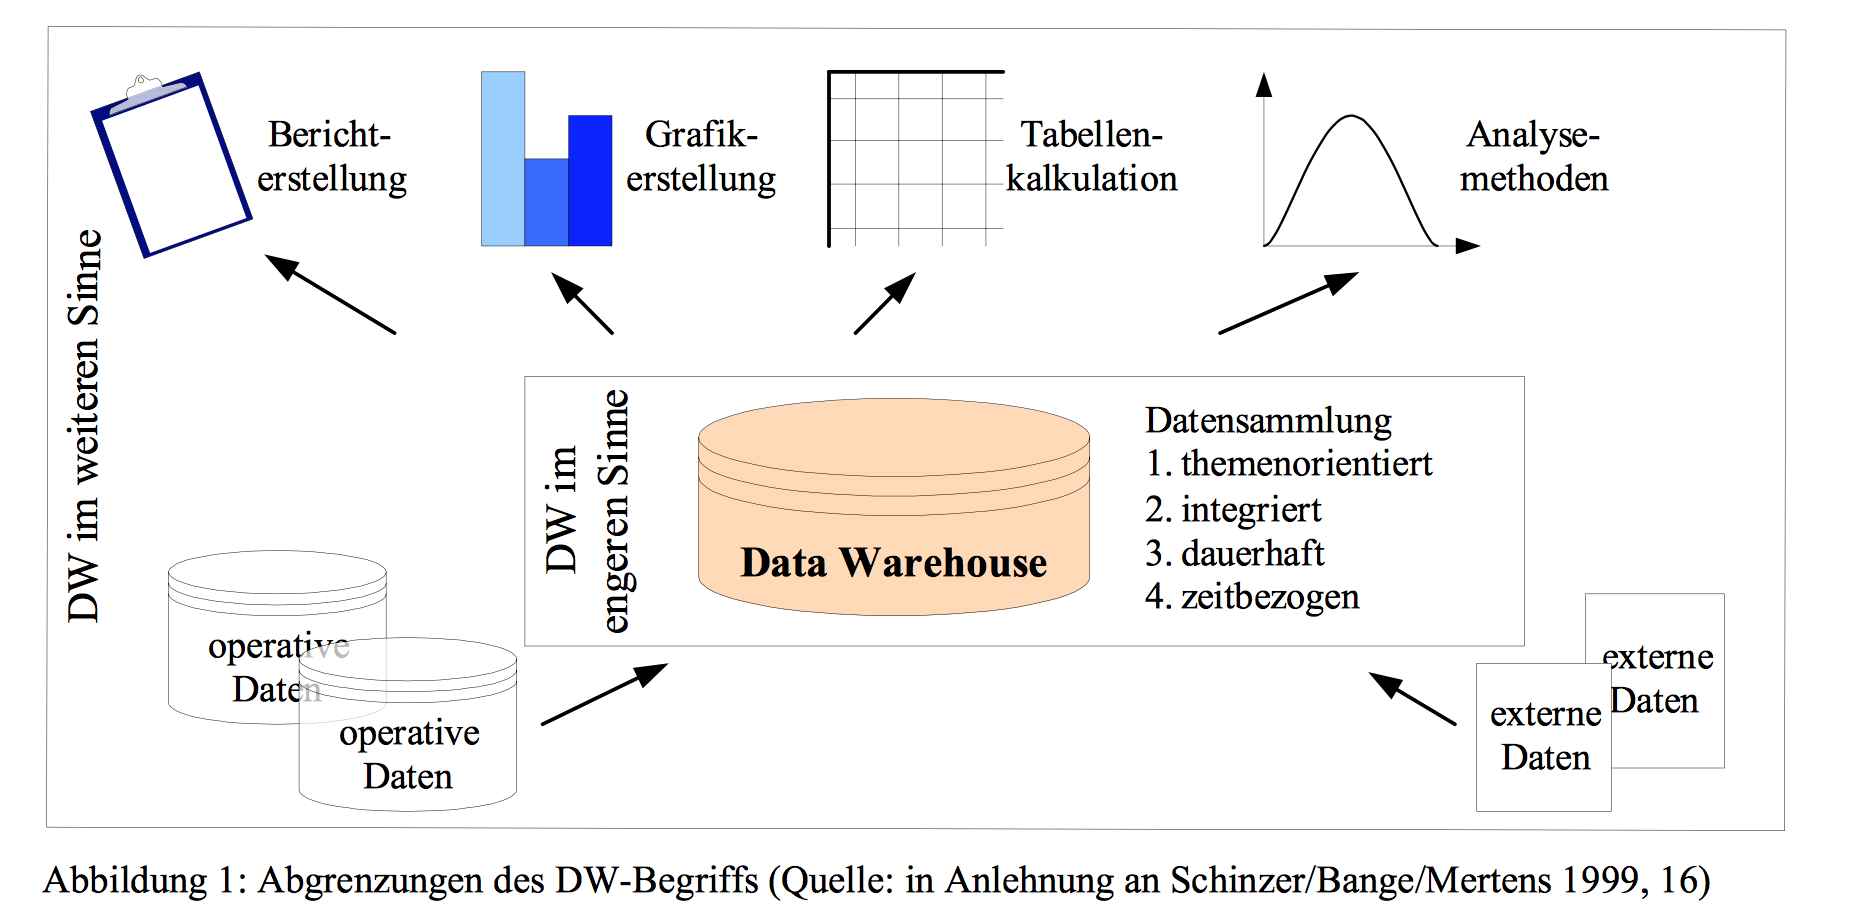
\includegraphics[width=1\textwidth]{files/DWOverview}
    \caption{Abgrenzungen des DW-Begriffs Q:(Schinzer/Bange/Mertens 1999, S.16)}
    \label{pic:DWOverview}
\end{figure}



%\section{SAP}
%\label{Kapitel:Einleitung}

%SAP NetWeaver Business Intelligence (kurz: SAP BI) (vormals: Business Information Warehouse, kurz BW) ist die Data-Warehouse-Anwendung (kurz DW) der SAP AG und Teil von SAP NetWeaver. BW besteht unter anderem aus Komponenten zum Datenmanagement (Data Warehousing Workbench), zur Definition von Benutzerabfragen über einen OLAP-Prozessor (Business Explorer, kurz BEx), aus einer Data-Mining-Umgebung (Analyseprozessdesigner, kurz APD) und einer Komponente zur Kontrolle der Ladeprozesse. Die derzeitige Version des SAP Business Intelligence hat die Releasenummer 7.3 und ist Teil des SAP NetWeaver 7.3. 
%Q: \url{http://de.wikipedia.org/wiki/SAP_NetWeaver_Business_Intelligence}